\documentclass[10pt]{book}
\usepackage{cdtBook}
\usepackage{cambios}
\usepackage{usecases}


%\newcommand{\proceso}{Gestión Integral de Residuos Sólidos Urbanos }
\defSistema{SIDAM}

\title{\Sistema \\\LARGE{sistema de rex \\{\bf Prototipo 1}}}
\subtitle{Análisis de Requerimientos}
%\author{}

%\date{martes 11 de mayo de 2010}

%%%%%%%%%%%%%%%%%%%%%%%%%%%%%%%%%%%%%%%%%%%%%%%%%%%%%%%%%%%%%%%%
\begin{document}
\ThisLRCornerWallPaper{0.5}{images/agua.png}
\maketitle\thispagestyle{empty}

\frontmatter
\tableofcontents

\mainmatter


%=========================================================
\chapter{Alcance del prototipo}

	En este capítulo se describe el alcance del prototipo a desarrollar. El alcance del sistema se ha definido como se muestra en la figura~\ref{fig:cu}.
	
\begin{figure}[htbp!]
	\begin{center}
		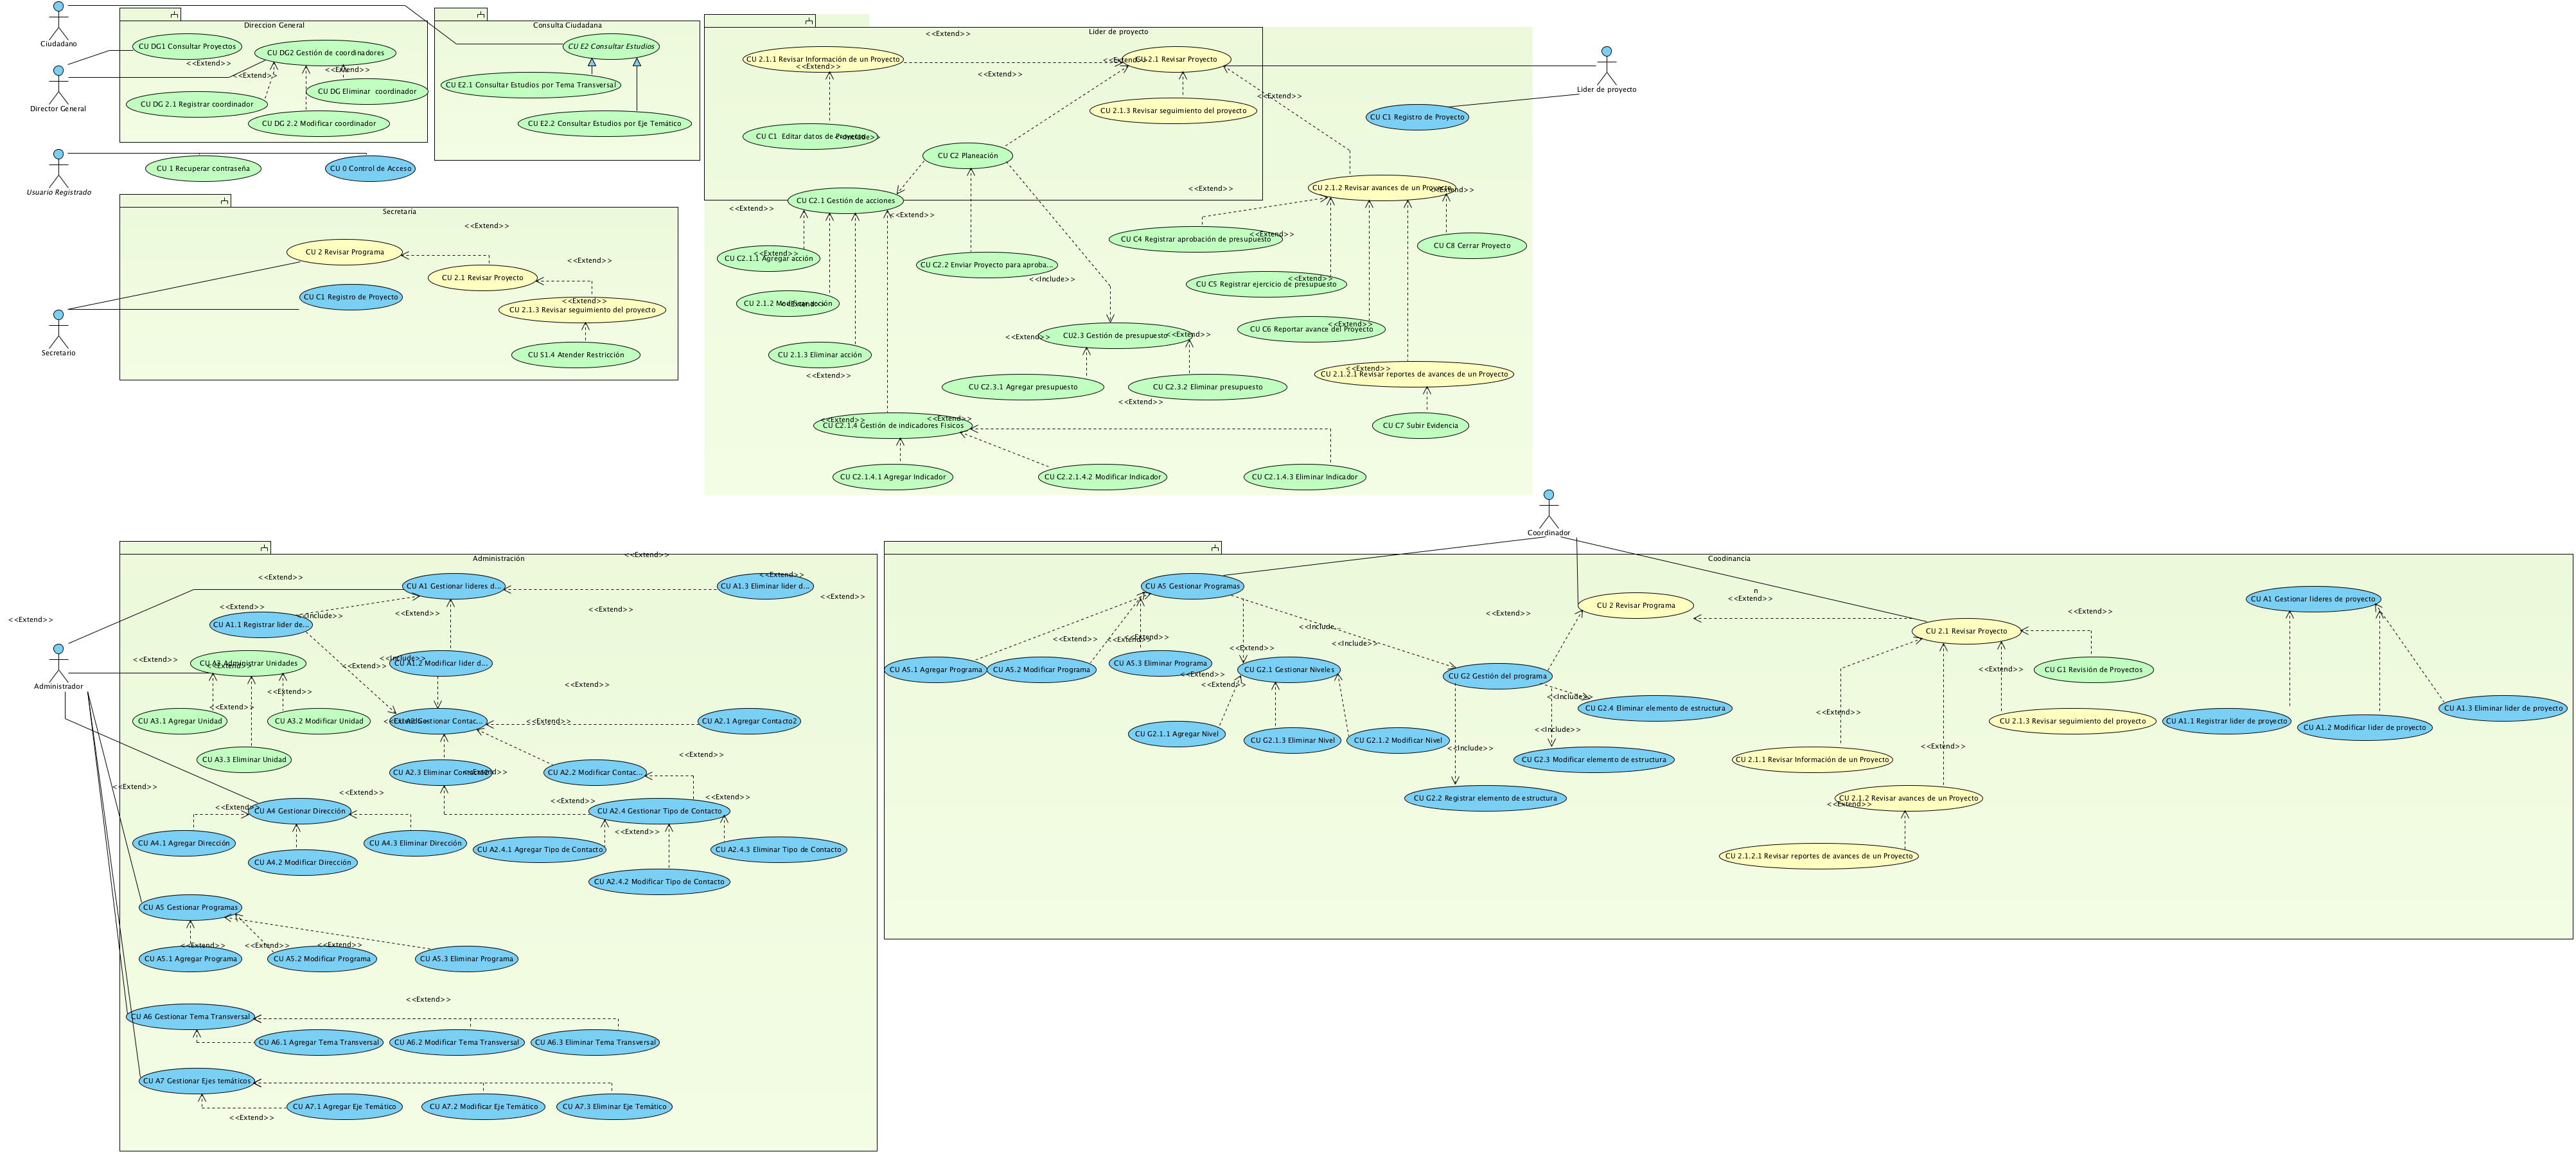
\includegraphics[width=.5\textwidth]{images/casosDeUso}
		\caption{Casos de uso.}
		\label{fig:cu}
	\end{center}
\end{figure}

\section{Actores}

El sistema será usado por los usuarios cuyos perfiles se describen en la figura~\ref{fig:actores}.

\begin{figure}[htbp!]
	\begin{center}
		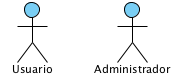
\includegraphics[width=.5\textwidth]{images/actores}
		\caption{Definición de actores del sistema.}
		\label{fig:actores}
	\end{center}
\end{figure}

%---------------------------------------------------------

\section{Requerimientos funcionales}
	%TODO Definir los datos de asistencia y nomina
	%TODO Definir lo que es la lista de asistencia, lo que es un recibo de nomina
	\begin{requerimientos}
		\FRitem{RF1}{Registro de datos de asistencia y nomina}{Se deben ingresar los datos de asistencia y nomina en forma de un archivo de excel.}{}
		\FRitem{RF2}{Registro de reportes de actividades}{Se ingresan los reportes de actividades de los empleados. Se debe asociar cada reporte con cada empleado.}{}
		\FRitem{RF3}{Generacion de lista de asistencia y recibos de nomina}{Se debe generar la lista de asistencia y los recibos de nomina con base en los datos de asistencia y nomina ingresados.}{}
	\end{requerimientos}



%=========================================================
\chapter{Proceso de negocios}


%---------------------------------------------------------
\section{Proceso}

\begin{figure}[htbp!]
	\begin{center}
		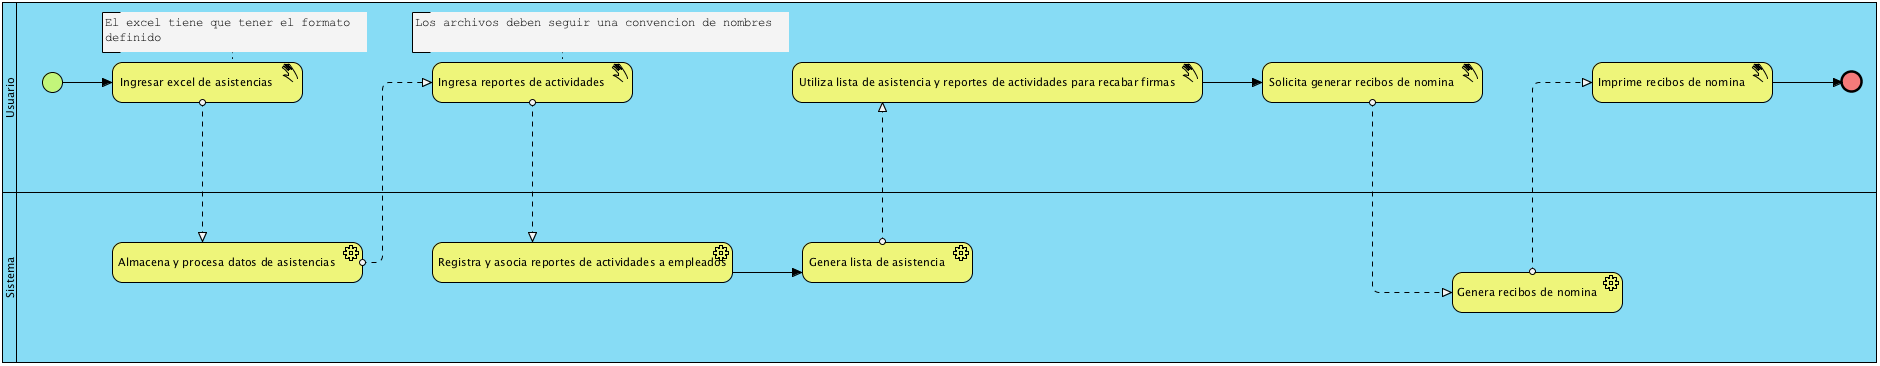
\includegraphics[width=.8\textwidth]{images/proceso}
		\caption{Proceso para la generacion de recibos de nomina.}
		\label{fig:recibosNomina}
	\end{center}
\end{figure}

%---------------------------------------------------------
\section{Reglas de Negocio}

\Instrucciones{Reglas de negocio: definición, hecho, afirmacion sobre un echo, restriccion, cálculo.}
\cfinput{reglas}


%=========================================================
\chapter{Modelo del comportamiento}

%---------------------------------------------------------
\section{Diagrama de CU}

\begin{figure}[htbp!]
	\begin{center}
		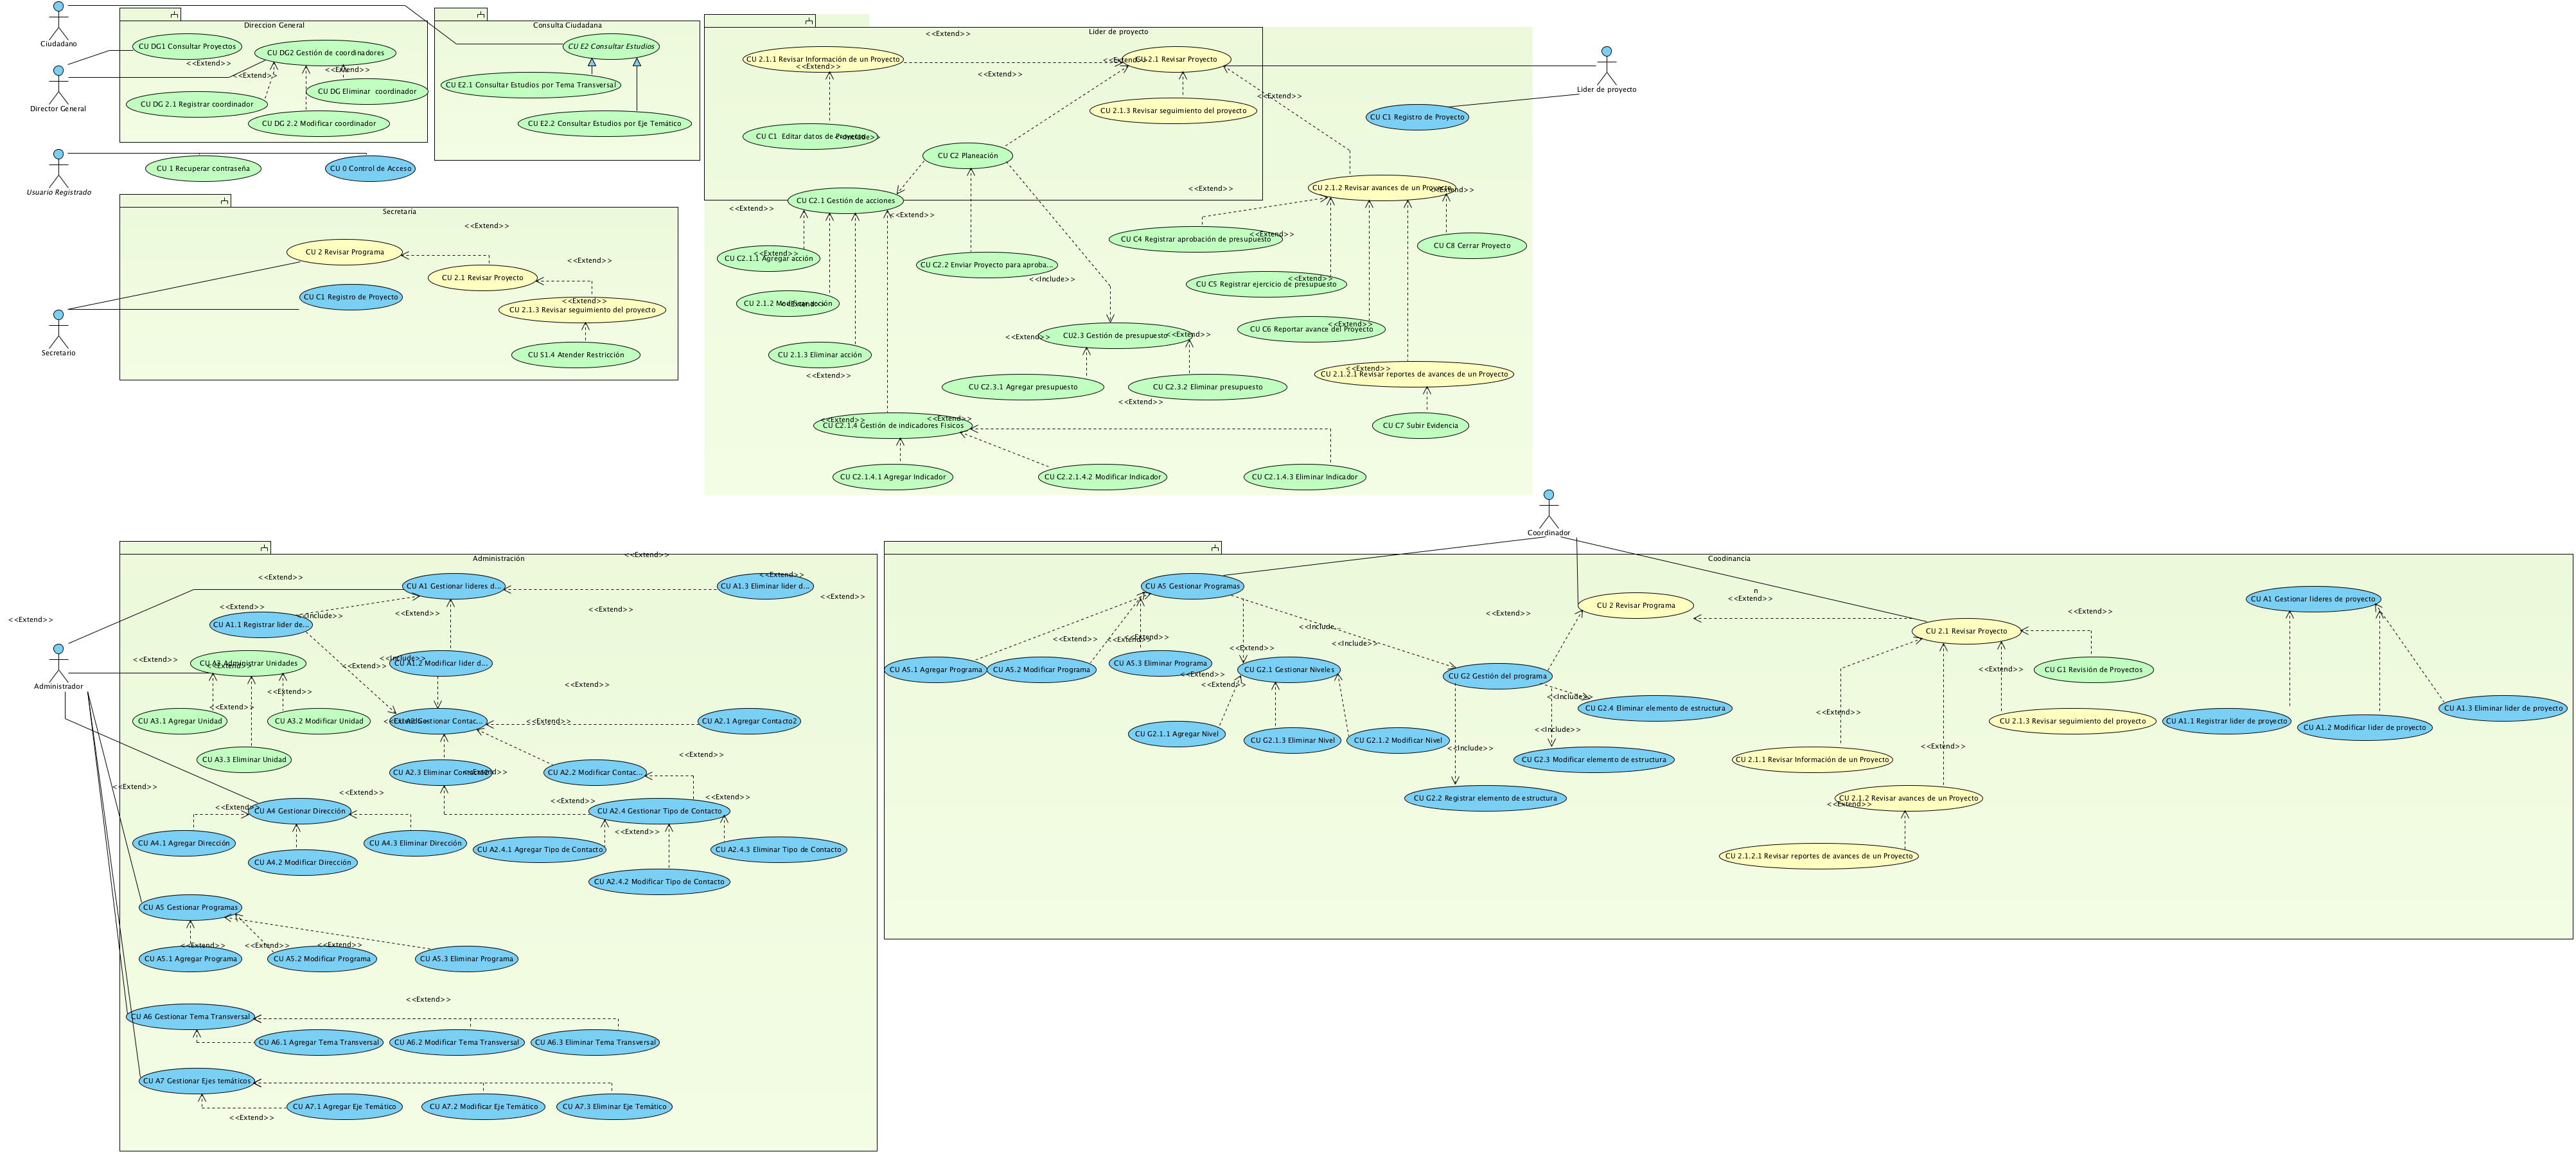
\includegraphics[angle=90,height=\textheight]{images/casosDeUso}
		\caption{Casos de uso del prototipo}
		\label{fig:default}
	\end{center}
\end{figure}

%=========================================================
\chapter{Modelo detallado del comportamiento, Control de acceso} 

%----------------------------------------------------------
\section{Diagrama de casos de uso}

\begin{figure}[htbp!]
	\begin{center}
		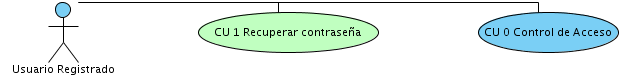
\includegraphics[width=.3\textwidth]{images/CUcontrolAcceso}
		\caption{Casos de uso para el control de acceso}
		\label{fig:default}
	\end{center}
\end{figure}

\cfinput{cu0iniciar_sesion/cu}


%%======================================================================\chapter{Modelo del dominio del problema} 

\section{Diagrama Entidad/Relación}

  	\begin{figure}[h!]
 		\centering
 			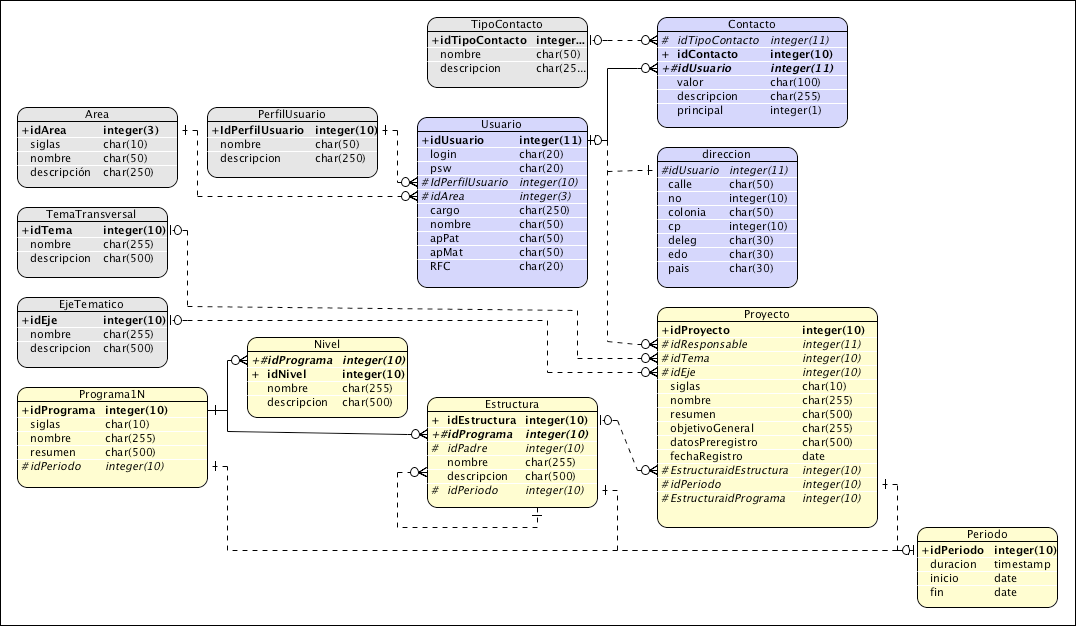
\includegraphics[width=.8\textwidth]{images/modeloER}
 		\caption{Unidad}
 	\end{figure}

\section{Diccionario de Datos}

\cfinput{diccionario}



\end{document}
